\documentclass[12pt, a4paper]{article}

% --- Packages ---
\usepackage[utf8]{inputenc}
\usepackage[T1]{fontenc}
\usepackage[english]{babel}
\usepackage{amsmath, amssymb}
\usepackage{graphicx}
\usepackage{booktabs}
\usepackage{hyperref}
\usepackage{natbib}
\usepackage{geometry}
\usepackage{caption}
\usepackage{subcaption}
\usepackage{float}
\usepackage{microtype}
\usepackage{setspace}
\usepackage{abstract}

\geometry{margin=2.5cm}
\onehalfspacing
\hypersetup{colorlinks=true, linkcolor=black, citecolor=black, urlcolor=blue}
\graphicspath{{figures/en/}}

% --- Metadata ---
\title{Magnificent Seven and Market Efficiency:\\
Decomposing S\&P500 Returns Through\\
Concentration Analysis (2019--2024)}

\author{
  Giulio Parrinello\\
  \small Universit\`a degli Studi di Palermo\\
  \small Ingegneria Gestionale\\
  \small \texttt{giulioparrinello@mail.com}
}

\date{Version 2, 14 October 2026\\
\small (version 1: June 2026; the differences are described in Section~\ref{sec:revision})}

% --- Document ---
\begin{document}
\maketitle

\begin{abstract}
This paper measures how much of the S\&P500's return between 2019 and 2024 is due to seven large technology firms, the ``Magnificent Seven'' (Apple, Microsoft, NVIDIA, Amazon, Alphabet, Meta and Tesla). We use daily prices, the number of shares outstanding reported to the SEC to reconstruct historical market capitalizations, and the equal-weight ETF RSP as a concentration-neutral benchmark. The capitalization-weighted index (SPY, $+157.5\%$) outperformed its equal-weight version (RSP, $+112.9\%$) by $44.6$ percentage points. Within the universe of the 50 largest stocks, rebuilt every year, the Magnificent Seven's share of market capitalization rises from $29.5\%$ to $55.0\%$, and the seven stocks account for $66\%$ of the cumulative return of this universe ($129.9$ of $196.9$ points). The mean daily return difference between SPY and RSP is not statistically significant ($p = 0.29$). This is version 2 of the paper: it corrects an error in the market capitalization calculation of version 1.
\end{abstract}

\section{Introduction}

The S\&P500 is regarded as a diversified gauge of the U.S. equity market. It is, however, capitalization-weighted: each firm weighs in proportion to its market value, so the largest companies move the index more than the others. Between 2019 and 2024 a growing share of the index's weight became concentrated in seven technology firms: Apple, Microsoft, NVIDIA, Alphabet, Amazon, Meta and Tesla, known as the ``Magnificent Seven''.

The question of this paper is: \emph{how much of the S\&P500's 2019--2024 performance is due to these seven firms, and what does that imply for market efficiency?} We address it in three ways. First, we compare the capitalization-weighted index (SPY) with its equal-weight version (RSP): the gap between the two directly measures the effect of concentration. Second, we reconstruct the historical market capitalizations of the 50 largest stocks and build a counterfactual index without the Magnificent Seven. Third, we decompose the return by year and by firm. We discuss the results in light of the Efficient Market Hypothesis \citep{fama1970, fama1991}.

\section{Note on the revision (version 2)}
\label{sec:revision}

Re-reading the paper in October 2026, I compared the reconstructed market capitalizations with known market values and found an error in the calculation of version 1 (June 2026). Version 1 multiplied the closing price downloaded from Yahoo Finance by the number of shares outstanding from the same source. The price, however, is already adjusted for stock splits, while the share count is not. For every stock with a split after 2019, the market capitalization before the split was therefore divided by the split factor. At the end of 2018, version 1 valued Amazon at 38 billion dollars instead of 734, Alphabet at 36 instead of 727, NVIDIA at 2 instead of 81 and Apple at 187 instead of 749.

The error understated the weight of the Magnificent Seven in the first part of the period. This is why version 1 reported a concentration rising from $16\%$ to $58\%$, ``more than threefold''. With the corrected market capitalizations the share rises from $29.5\%$ to $55.0\%$: it almost doubled (Figure~\ref{fig:revision}). The results based only on ETFs (SPY, RSP, Sharpe ratios, drawdowns, the statistical test) did not depend on market capitalizations and change only slightly, because the period now also includes 31 December 2024.

\begin{figure}[H]
  \centering
  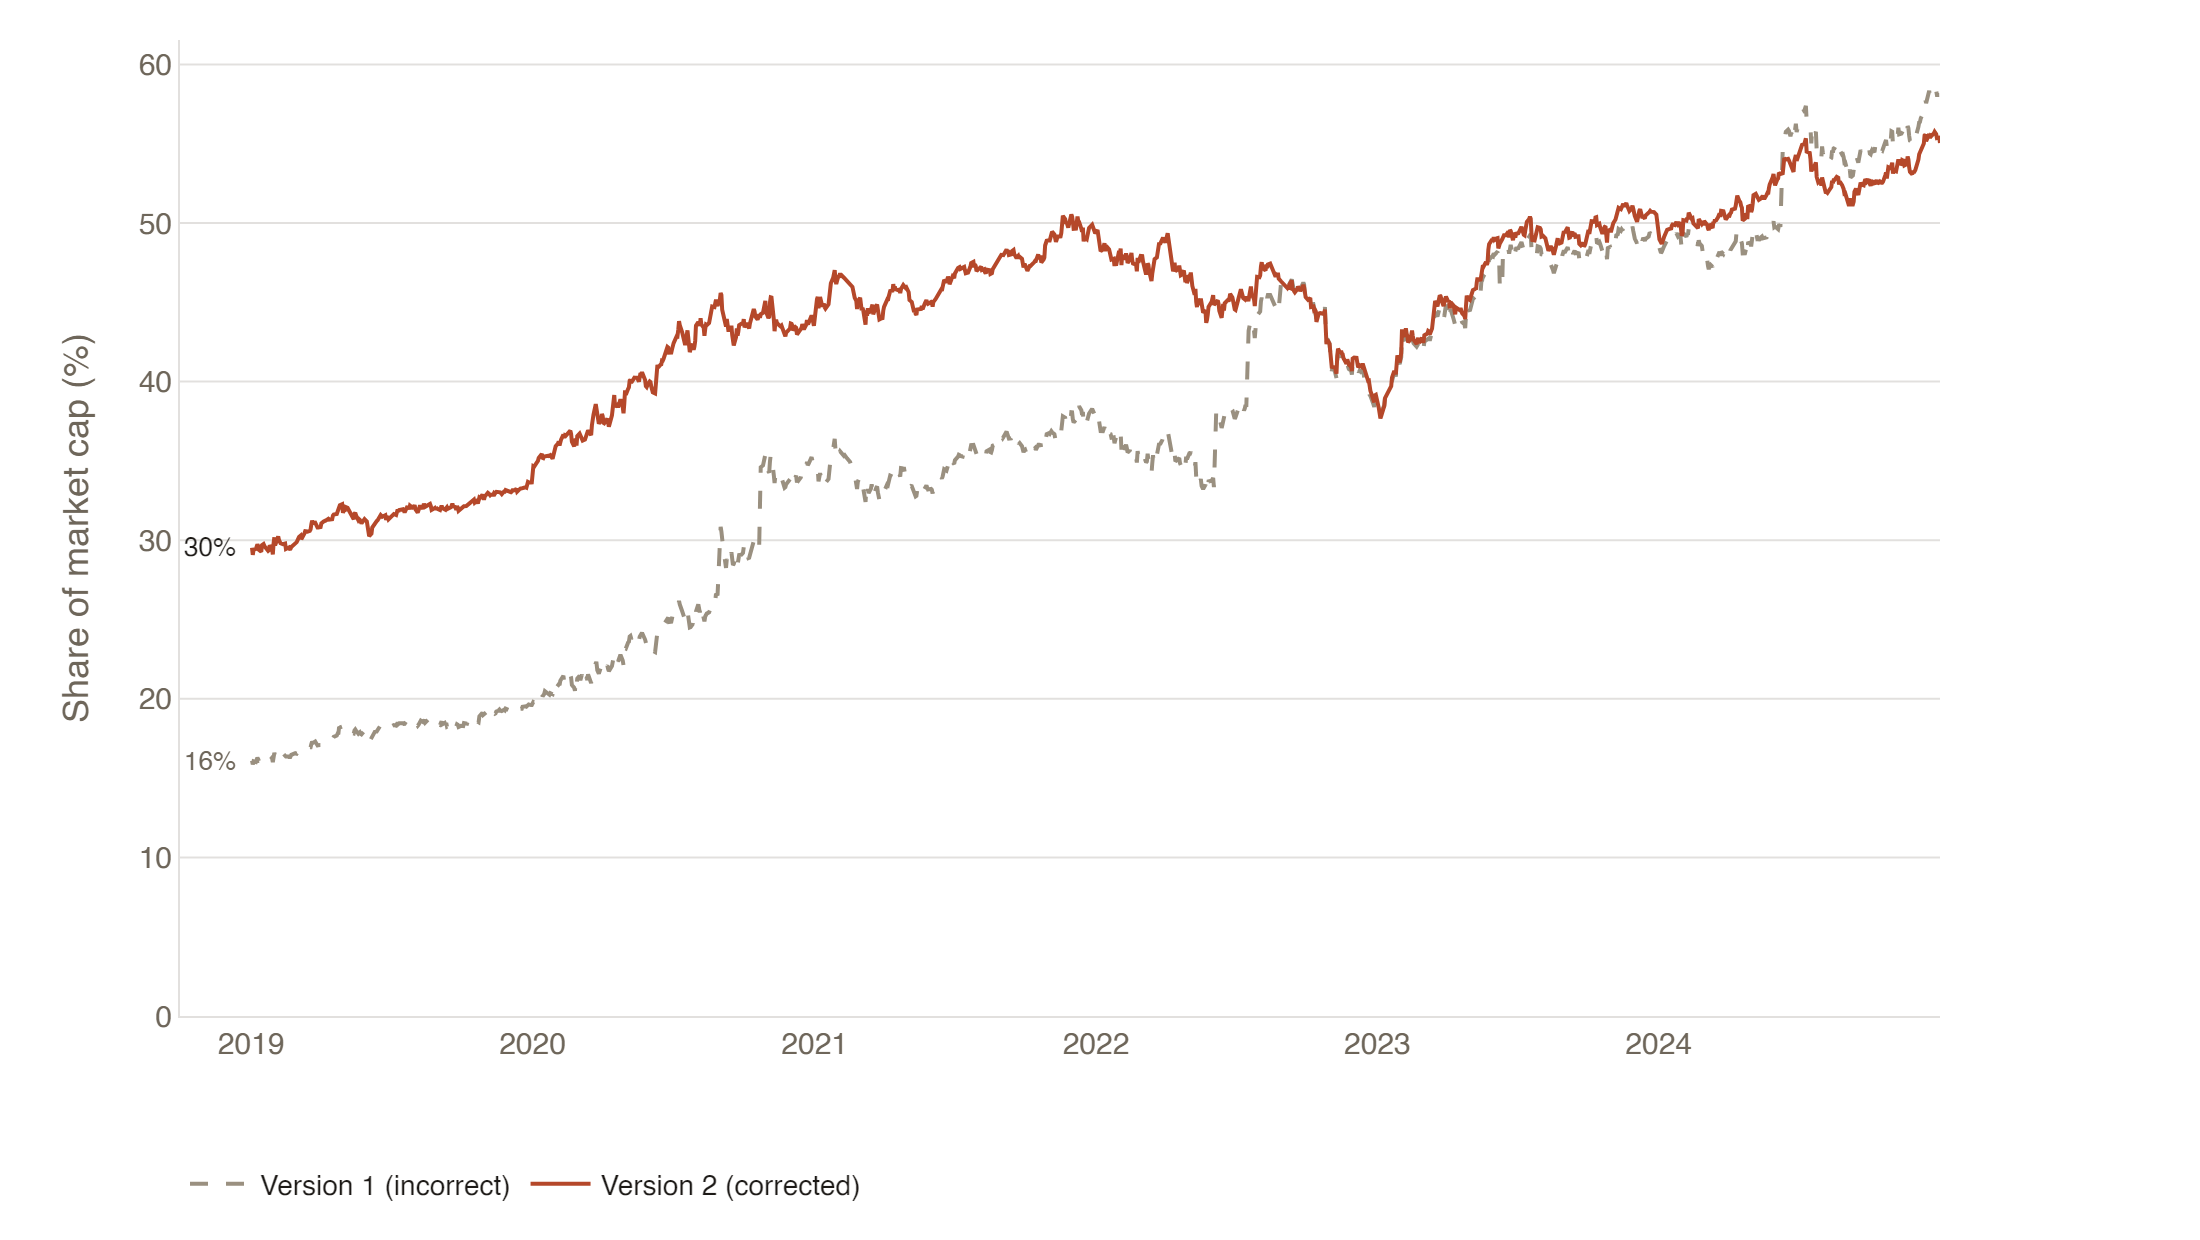
\includegraphics[width=\linewidth]{revision_chart.png}
  \caption{Share of the Magnificent Seven in the market capitalization of the 50 largest stocks: version 1 (incorrect) and version 2 (corrected). The two series converge after the Amazon (June 2022) and Alphabet (July 2022) splits, when the error no longer applies.}
  \label{fig:revision}
\end{figure}

Besides fixing the error, version 2 makes the following changes:
\begin{itemize}
  \item share counts come from filings with the SEC \citep{secedgar} and are put on the same split basis as the price;
  \item the universe of 50 stocks is rebuilt every year with the data available at the end of the previous year, instead of being chosen by average market capitalization over the whole period; Tesla enters only after joining the S\&P500 (21 December 2020);
  \item no data point is filled backwards with future values;
  \item each stock's contribution is computed with an exact attribution, whose contributions sum to the index return; version 1 instead reported a counterfactual comparison as the ``share of return'';
  \item the statistical test is repeated with autocorrelation-robust standard errors \citep{neweywest1987};
  \item the period ends on 31 December 2024 (version 1 stopped on 30 December because of how the end date was set);
  \item a source that could not be verified has been removed from the references.
\end{itemize}

\begin{table}[H]
  \centering
  \caption{Main results in the two versions.}
  \begin{tabular}{lrr}
    \toprule
    & Version 1 & Version 2 \\
    \midrule
    Mag7 share of top 50, start of 2019     & $16.1\%$  & $29.5\%$ \\
    Mag7 share of top 50, end of 2024       & $58.1\%$  & $55.0\%$ \\
    Share of return due to Mag7             & $35\%$\textsuperscript{a} & $66\%$\textsuperscript{b} \\
    Top 50 excluding Mag7, cumulative return & $+108.5\%$ & $+98.4\%$ \\
    Mag7 only, cumulative return            & $+364.7\%$ & $+416.6\%$ \\
    SPY, cumulative return                  & $+158.4\%$ & $+157.5\%$ \\
    RSP, cumulative return                  & $+112.5\%$ & $+112.9\%$ \\
    \bottomrule
  \end{tabular}
  \par\smallskip
  \footnotesize\textsuperscript{a} Difference between the index with and without Mag7, divided by the index return. \textsuperscript{b} Exact attribution (Section~\ref{sec:attribution}).
  \label{tab:revision}
\end{table}

The code, the data used (shares per stock and date, with their source) and the history of changes are public in the project repository (\url{https://github.com/giulioparrinello/sp500-concentration}), with instructions to replicate the results: version 1 is the first commit, version 2 the following ones.

\section{Literature review}

\subsection{The Efficient Market Hypothesis}

\citet{fama1970} proposed the classification of market efficiency into three forms. The semi-strong form holds that prices reflect all public information, so no investor can systematically earn abnormal returns through fundamental analysis. \citet{fama1991} later highlighted the joint-hypothesis problem: every test of efficiency is also a test of the assumed asset-pricing model.

\subsection{Behavioural critiques}

\citet{shiller1981} showed that stock prices move far more than subsequent changes in dividends would justify. \citet{debondt1985} documented systematic overreaction: the stocks that lost most over the previous three to five years later outperform those that gained most. Both results indicate that prices can drift away from fundamentals, especially in periods of strong enthusiasm.

\subsection{Concentration of stock returns}

\citet{bessembinder2018} shows that, in the U.S. market from 1926 to 2016, the net gain of stocks over short-term Treasury bills is due to a small minority of firms: about $4\%$ of listed companies account for all the net wealth created. Return concentration is therefore not new. The 2019--2024 period is of interest because the concentration involves a few stocks that were already very large and that, by construction, weigh heavily in the indices followed by passive investors. The classic argument for diversification goes back to \citet{markowitz1952}.

\section{Data and methodology}

\subsection{Data sources}

Daily prices come from Yahoo Finance through the Python library \texttt{yfinance}. SPY represents the capitalization-weighted S\&P500 and the Invesco RSP ETF its equal-weight version. The period runs from 2 January 2019 to 31 December 2024: $1{,}510$ trading days and $1{,}509$ daily returns. Returns use prices adjusted for splits and dividends; market capitalizations use the closing price adjusted for splits only.

Shares outstanding come from the XBRL data filed with the SEC \citep{secedgar}, taking for each date the first published value. For 98 firms we use the figure reported on the cover page of quarterly and annual reports (\texttt{EntityCommonStockSharesOutstanding}); for 10 firms for which that figure is not available in aggregate form over the whole period (for example Meta and Mastercard, which have several share classes) we use the quarterly weighted average of shares outstanding; for Alphabet, the total of its three classes from the balance sheet. For Visa and Berkshire Hathaway the SEC does not provide an aggregate total, and we use Yahoo Finance's equivalent share count (quarterly median). The risk-free rate is the 13-week T-bill yield (\texttt{\^{}IRX}).

\subsection{Historical market capitalizations}

The market capitalization of firm $i$ on day $t$ is
\begin{equation}
  m_{i,t} = p_{i,t}\, s_{i,t},
\end{equation}
where $p_{i,t}$ is the closing price and $s_{i,t}$ the number of shares, both on the same split basis. The share count is held constant until the next SEC figure. Three adjustments prevent systematic errors: figures already reported after a split but referring to an earlier date are brought back to the correct basis (this is the case for Alphabet in June 2022 and TJX in November 2018); for mergers that change the share count substantially (for example Celgene into Bristol-Myers Squibb, Allergan into AbbVie, Xilinx into AMD) the new count applies from the closing date of the deal; spin-offs (for example WarnerMedia from AT\&T and GE HealthCare from General Electric) reduce the market capitalization from the distribution date. An automatic check verifies that, outside these events, market capitalization never moves more than the price by over $15\%$ in a day. The resulting market capitalizations match known market values: at the end of 2024 Apple is worth $3{,}785$ billion dollars, NVIDIA $3{,}289$, Microsoft $3{,}134$.

\subsection{Universe and reconstructed index}

We start from 111 candidate firms, all those that could rank among the 50 largest in the S\&P500 during the period. On the last trading day of each year we select the 50 with the highest market capitalization, considering only firms already in the index, and keep them for the whole following year. The entry threshold, i.e.\ the market capitalization of the fiftieth firm, ranges from $91$ billion dollars at the end of 2018 to $176$ billion at the end of 2021. In total, 66 firms enter the universe for at least one year. NVIDIA is excluded in 2019 (81 billion at the end of 2018) and Tesla enters from 2021.

The reconstructed index is capitalization-weighted with the previous day's weights:
\begin{equation}
  r_t = \sum_{i \in U_t} w_{i,t-1}\, r_{i,t}, \qquad w_{i,t-1} = \frac{m_{i,t-1}}{\sum_{j \in U_t} m_{j,t-1}},
\end{equation}
where $U_t$ is the universe for the year of $t$. Its daily return has a correlation of $0.974$ with SPY's, with an annualized tracking error of $4.9$ percentage points: the 50-stock universe follows the index closely but does not replicate it. The counterfactual index ``excluding the Magnificent Seven'' uses the same formula, removing the seven stocks and spreading their weight over the others.

\subsection{Return attribution}
\label{sec:attribution}

The contribution of firm $i$ to the index's cumulative return is
\begin{equation}
  C_i = \sum_{t} w_{i,t-1}\, r_{i,t}\, \frac{I_{t-1}}{I_0},
\end{equation}
where $I_t$ is the index level. With this definition the contributions sum exactly to the index's cumulative return. The annual contribution uses the same formula, with the index level at the start of the year in place of $I_0$.

\subsection{Risk-adjusted performance}

The annualized Sharpe ratio is computed over the whole period and over a rolling 252-day window, using the realized risk-free rate, which went from near zero in 2020--2021 to over $5\%$ in 2023--2024:
\begin{equation}
  \mathrm{Sharpe} = \frac{\overline{r_t - r^{f}_t}}{\sigma(r_t - r^{f}_t)} \, \sqrt{252}.
\end{equation}

\subsection{Limitations}

\begin{itemize}
  \item The universe includes only the 50 largest stocks: shares and contributions refer to this universe, not to the whole S\&P500, where the Magnificent Seven weigh less.
  \item The candidates are 111 firms chosen among the largest of the period; a firm missing from the list that exceeded the entry threshold would be missing from the universe.
  \item We use total market capitalization, while the S\&P500 weights firms by their freely tradable shares (free float).
  \item Share counts are updated once per quarter; for Visa and Berkshire Hathaway the source is Yahoo Finance rather than the SEC.
  \item SPY and RSP are funds that track the indices, with a small tracking error and different fees.
  \item The Magnificent Seven group is defined ex post, as the set of firms that ended up dominating the index.
  \item The period includes exceptional events (the 2020 crash, the subsequent recovery and the 2022 rate rise) that amplify the measured effect.
\end{itemize}

\section{Results}

\subsection{Performance comparison}

\begin{figure}[H]
  \centering
  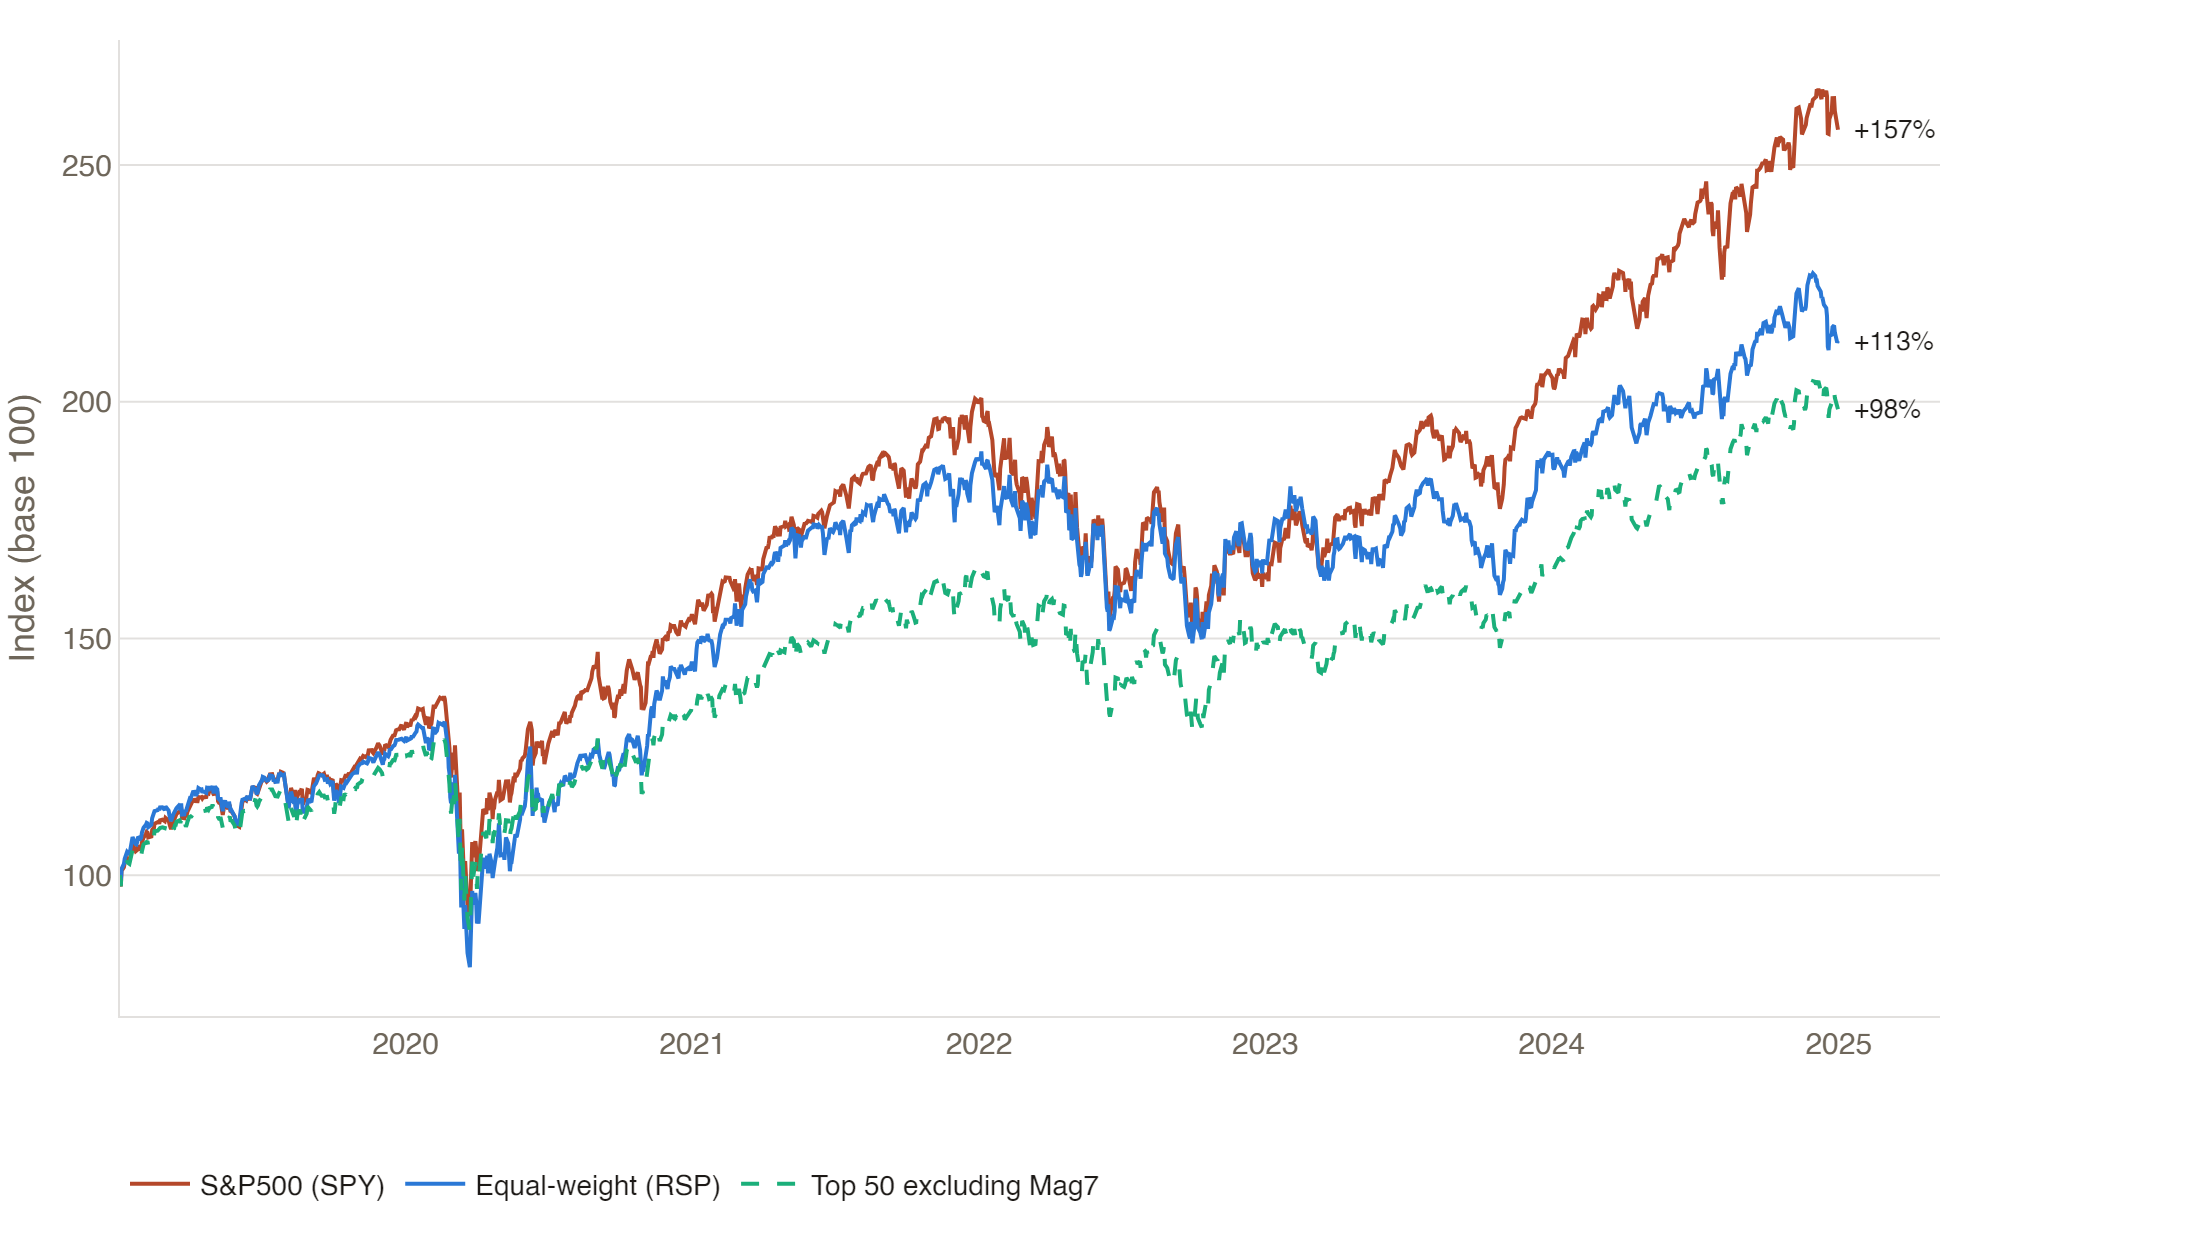
\includegraphics[width=\linewidth]{performance_chart.png}
  \caption{Cumulative performance (base $=100$) of SPY, RSP and the reconstructed index of the 50 largest stocks excluding the Magnificent Seven, 2019--2024.}
  \label{fig:performance}
\end{figure}

SPY returned $+157.5\%$ over the period and RSP $+112.9\%$: a gap of $44.6$ percentage points (Figure~\ref{fig:performance}). The index of the 50 largest stocks excluding the Magnificent Seven returned $+98.4\%$. The three curves stay close until spring 2020 and then diverge. SPY's lead is not constant: RSP did better in 2021 ($+29.4\%$ against $+28.7\%$) and in 2022 ($-11.6\%$ against $-18.2\%$), while in 2023 and 2024 SPY returned about twice as much as RSP ($+26.2\%$ against $+13.7\%$ and $+24.9\%$ against $+12.8\%$).

\subsection{Return attribution}

\begin{figure}[H]
  \centering
  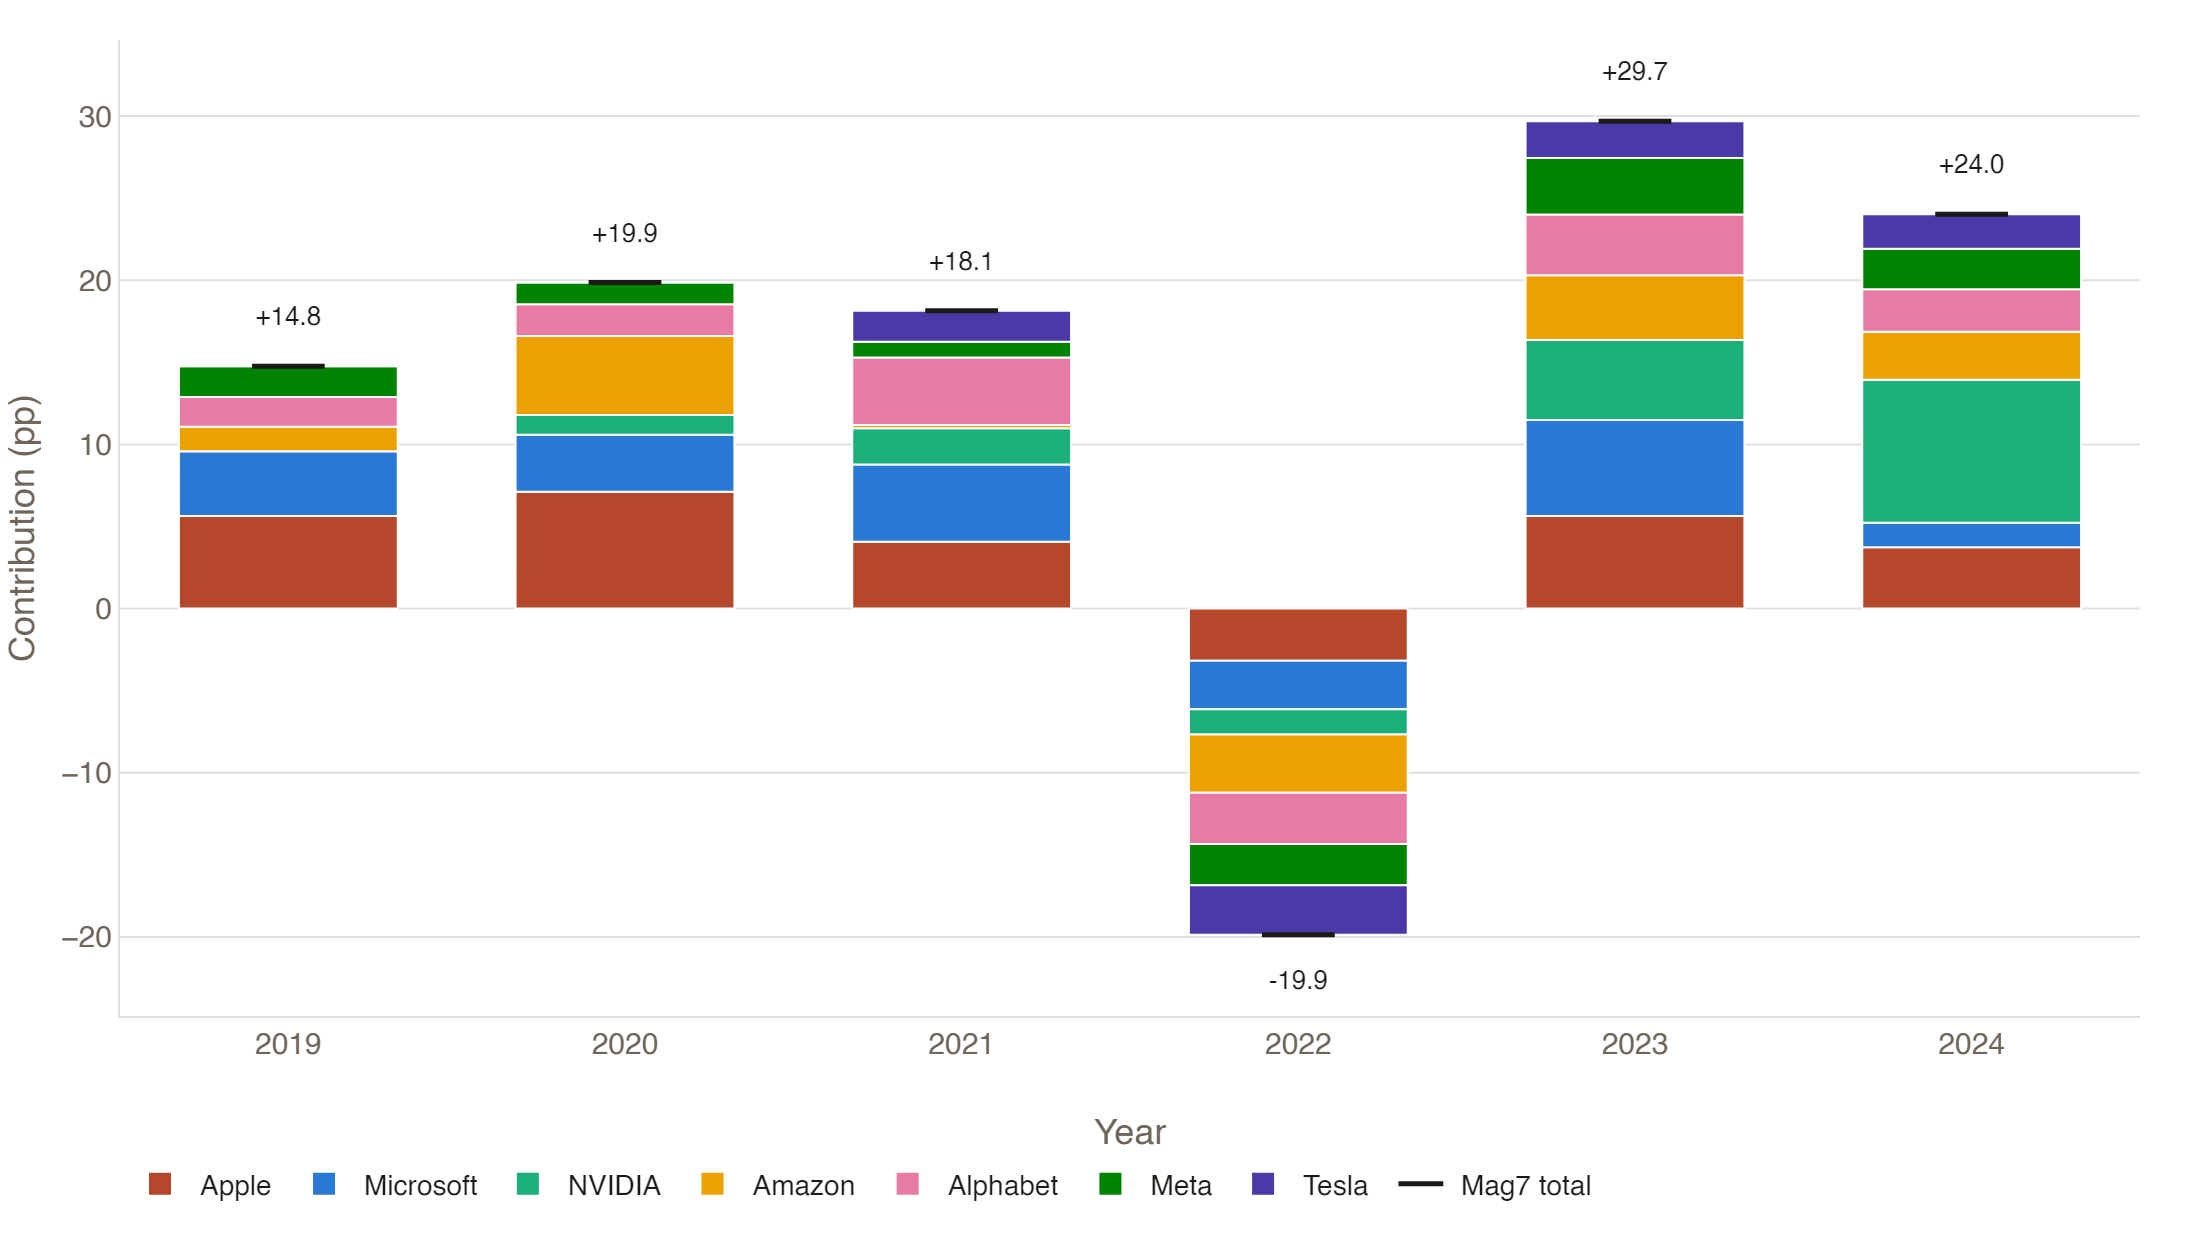
\includegraphics[width=\linewidth]{attribution_chart.png}
  \caption{Annual contribution of each Magnificent Seven stock to the return of the index of the 50 largest stocks (percentage points). The black segment marks the total of the seven stocks. NVIDIA is not part of the universe in 2019, Tesla in 2019 and 2020.}
  \label{fig:attribution}
\end{figure}

Over the whole period the 50-stock index returned $+196.9\%$ and the Magnificent Seven account for $129.9$ points of it, i.e.\ $66\%$. By firm: Apple $32.4$ points, NVIDIA $29.1$, Microsoft $22.8$, Alphabet $16.2$, Amazon $13.5$, Meta $10.9$, Tesla $4.9$. The contribution varies widely from year to year (Figure~\ref{fig:attribution}): the seven stocks add $14.8$ points out of $32.6$ in 2019 and $29.7$ out of $36.3$ in 2023, while in 2022 they subtract $19.9$ points out of a total loss of $24.6$. Over 2023--2024 the largest contribution comes from NVIDIA ($13.6$ points), followed by Apple ($9.4$), Microsoft ($7.3$), Amazon ($6.9$), Alphabet ($6.3$), Meta ($5.9$) and Tesla ($4.3$). In 2024 alone NVIDIA adds $8.7$ points, more than any other stock in any single year of the period.

The counterfactual comparison leads to the same conclusion: without the Magnificent Seven the 50-stock index would have returned $+98.4\%$ instead of $+196.9\%$.

\begin{table}[H]
  \centering
  \caption{Main metrics, 2019--2024. Sharpe ratios use the realized 13-week T-bill rate. ``Excl.\ Mag7'' and ``Mag7 only'' are built on the universe of the 50 largest stocks.}
  \begin{tabular}{lrrrr}
    \toprule
    & SPY & RSP & Excl.\ Mag7 & Mag7 only \\
    \midrule
    Cumulative return       & $157.5\%$ & $112.9\%$ & $98.4\%$  & $416.6\%$ \\
    Annualized return       & $17.1\%$  & $13.4\%$  & $12.1\%$  & $31.5\%$ \\
    Annualized volatility   & $19.8\%$  & $20.9\%$  & $18.2\%$  & $28.3\%$ \\
    Sharpe ratio            & $0.77$    & $0.59$    & $0.59$    & $1.03$ \\
    Maximum drawdown        & $-33.7\%$ & $-39.0\%$ & $-31.5\%$ & $-44.0\%$ \\
    \bottomrule
  \end{tabular}
  \label{tab:metrics}
\end{table}

On their own, the Magnificent Seven have a Sharpe ratio of $1.03$, higher than SPY ($0.77$) and RSP ($0.59$), with higher volatility ($28.3\%$) and a deeper maximum drawdown ($-44.0\%$) (Table~\ref{tab:metrics}). SPY's Sharpe ratio advantage over RSP therefore comes from the weight SPY gives to these stocks.

\subsection{Concentration over time}

\begin{figure}[H]
  \centering
  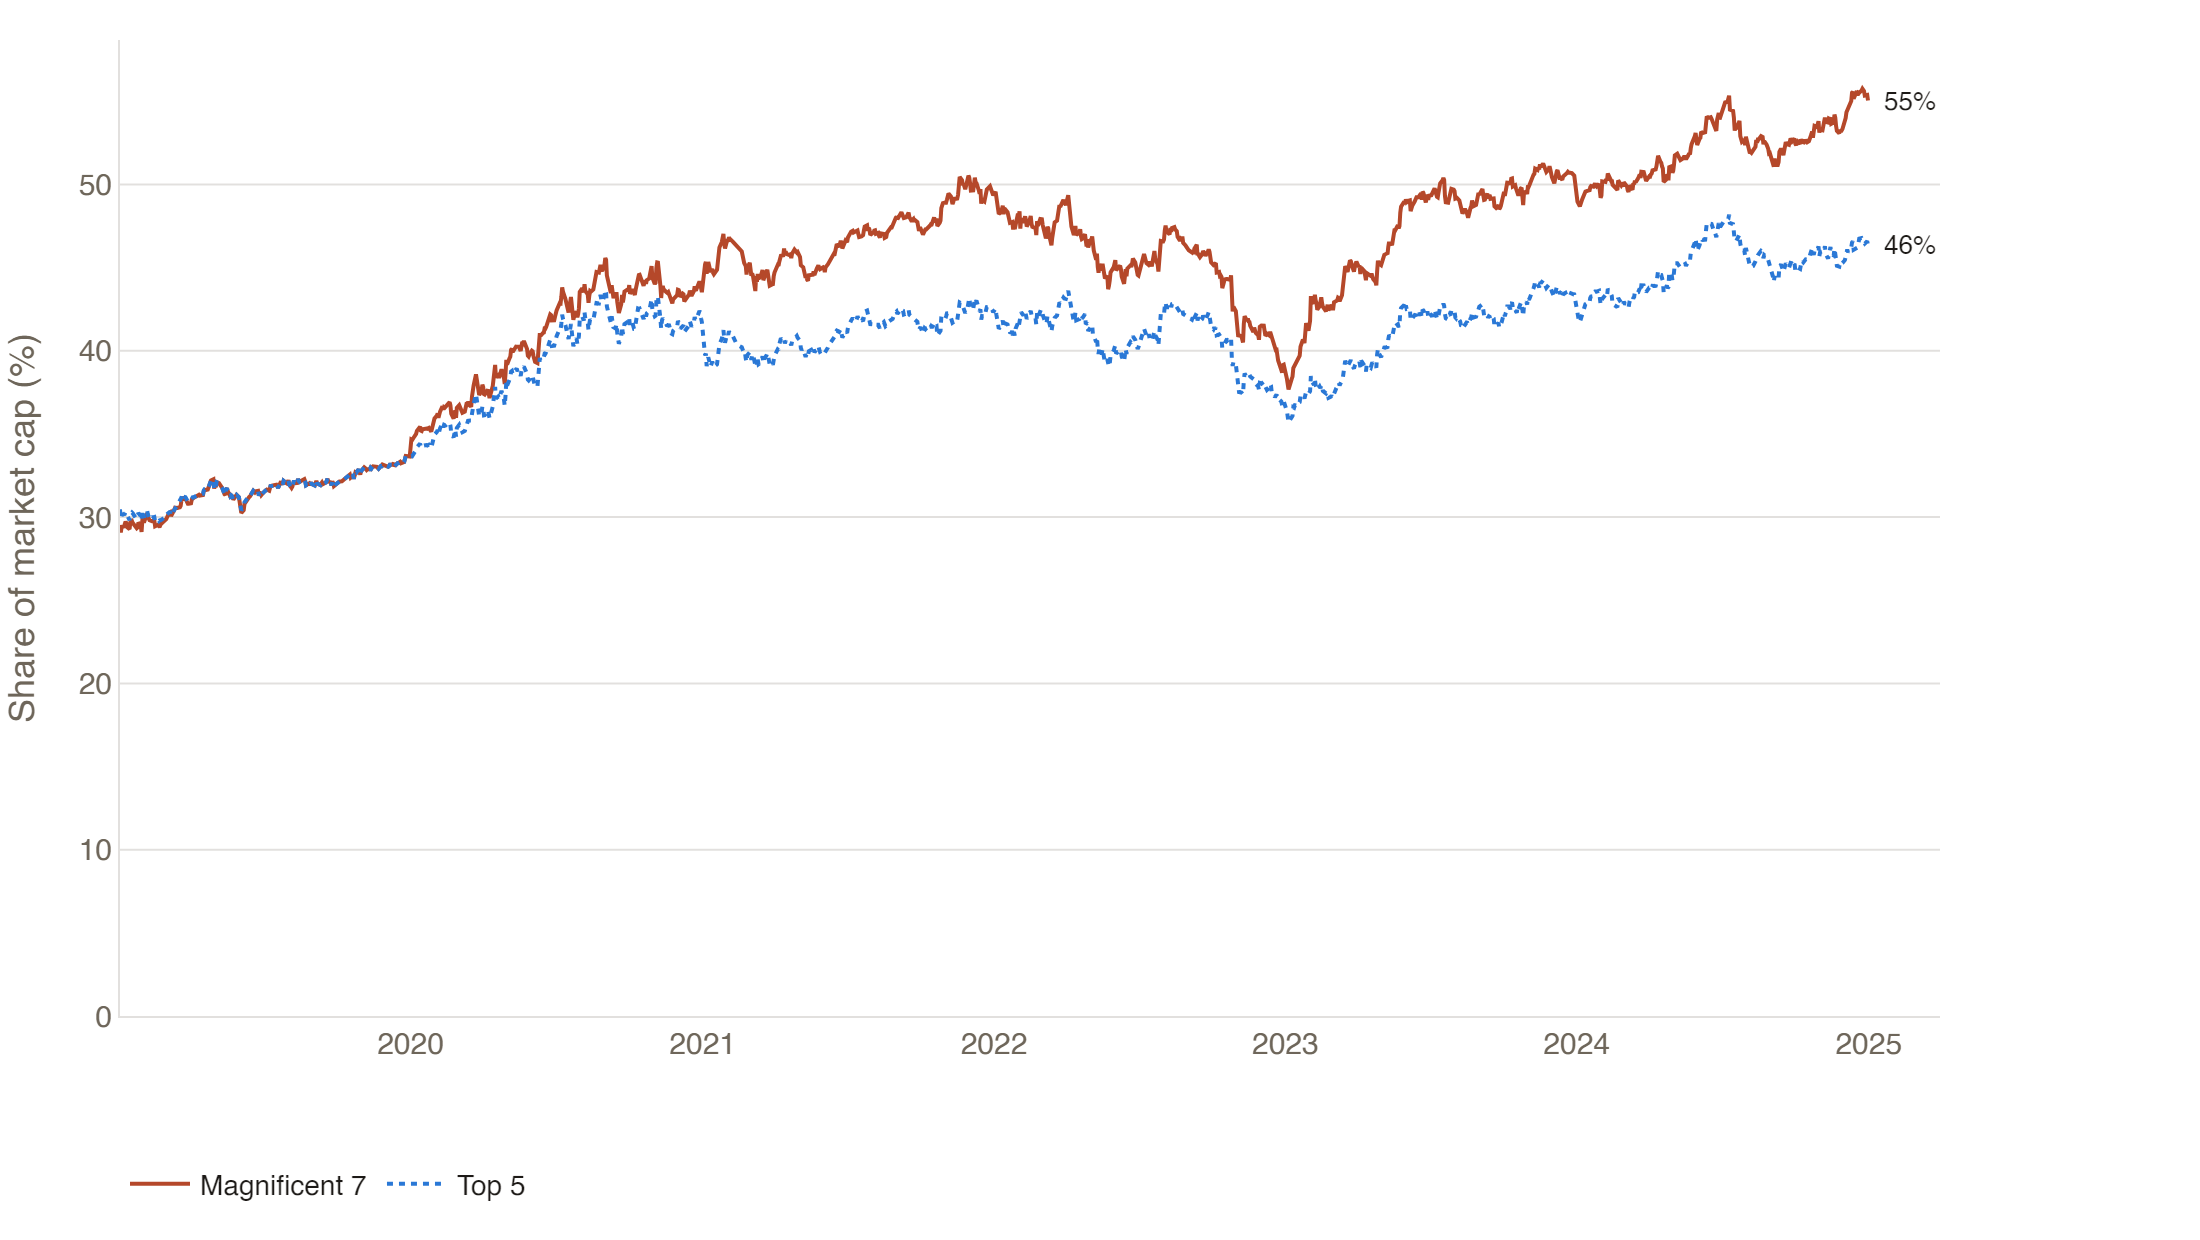
\includegraphics[width=\linewidth]{concentration_chart.png}
  \caption{Share of the Magnificent Seven and of the five largest stocks in the market capitalization of the universe of the 50 largest stocks, 2019--2024.}
  \label{fig:concentration}
\end{figure}

The Magnificent Seven's share of the market capitalization of the 50 largest stocks rises from $29.5\%$ at the start of 2019 to $55.0\%$ at the end of 2024, peaking at $55.8\%$ on 24 December 2024 (Figure~\ref{fig:concentration}). The rise stops in 2022: the share falls to $37.7\%$ on 5 January 2023 and then recovers. The five largest stocks go from $30.5\%$ to $46.4\%$ of the universe. The small jumps at the start of each year reflect the rebuilding of the universe (for example NVIDIA entering in 2020 and Tesla in 2021).

\subsection{Correlation structure}

\begin{figure}[H]
  \centering
  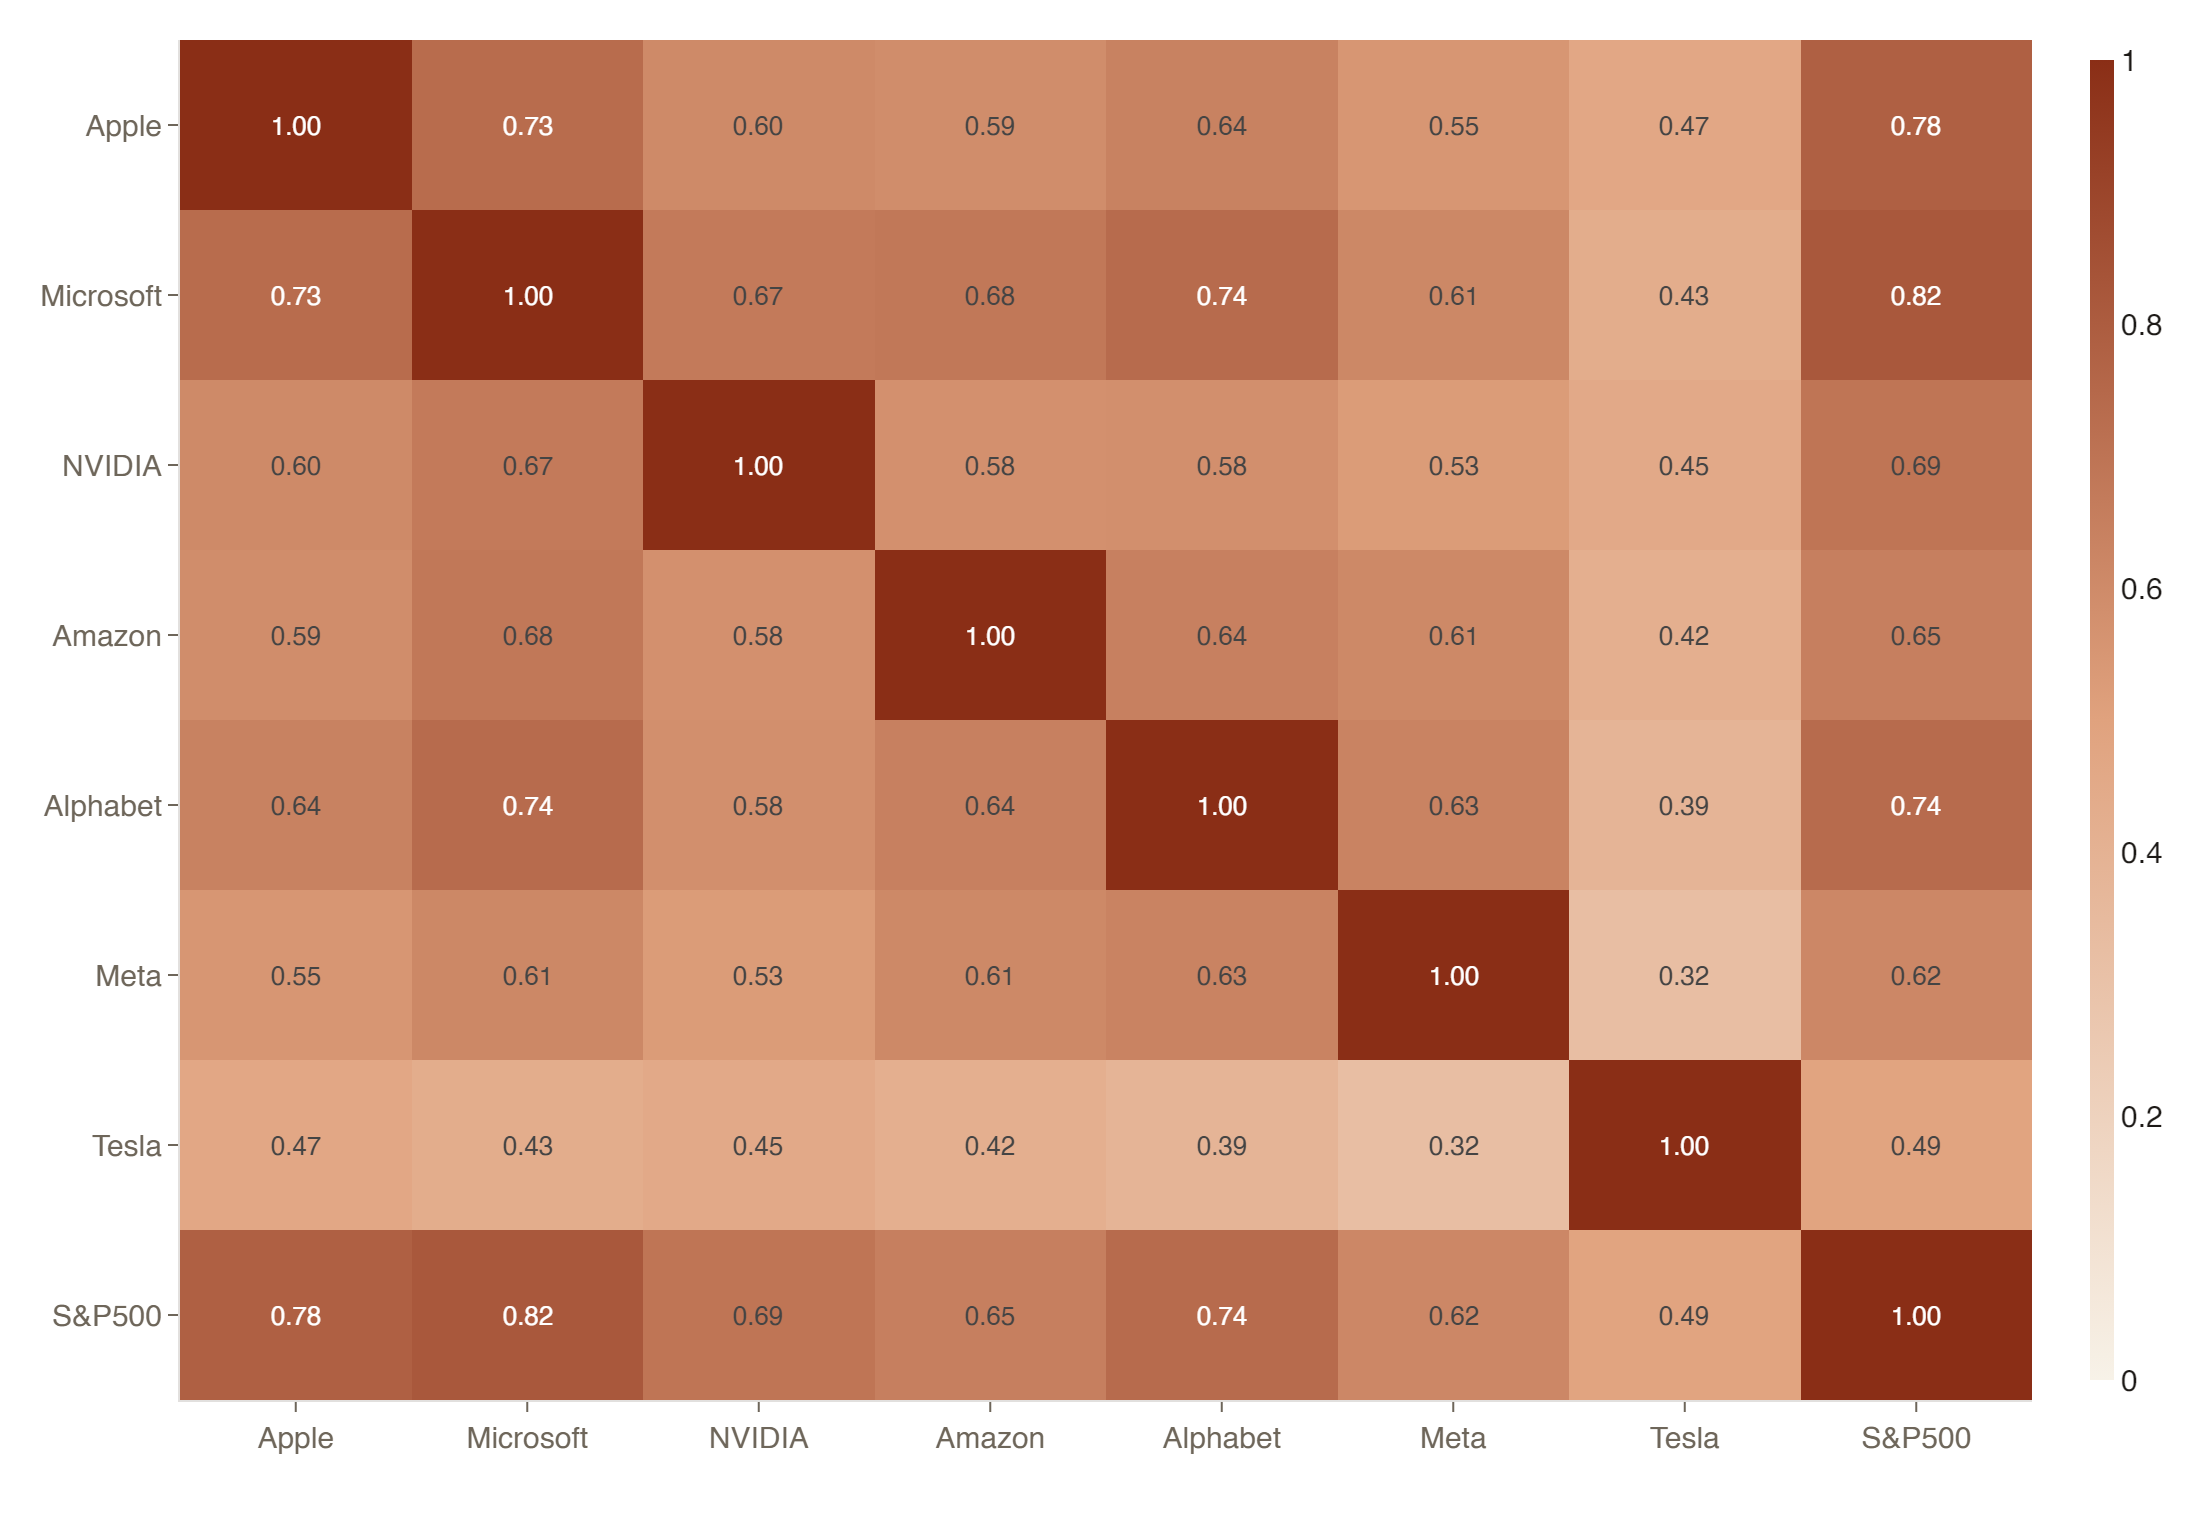
\includegraphics[width=0.85\linewidth]{heatmap_chart.png}
  \caption{Pearson correlation of daily returns between the Magnificent Seven and the S\&P500 (SPY), 2019--2024.}
  \label{fig:heatmap}
\end{figure}

The average correlation between the daily returns of the Magnificent Seven and those of SPY is $0.68$ (Figure~\ref{fig:heatmap}). Among the seven stocks, correlations range from $0.32$ to $0.74$; Tesla is the stock least related to the others and to the index ($0.49$ with SPY). The more these stocks weigh in the index, the more their correlation with the index rises by construction: an index holder owns a growing share of technology stocks that are correlated with each other.

\subsection{Risk-adjusted performance}

\begin{figure}[H]
  \centering
  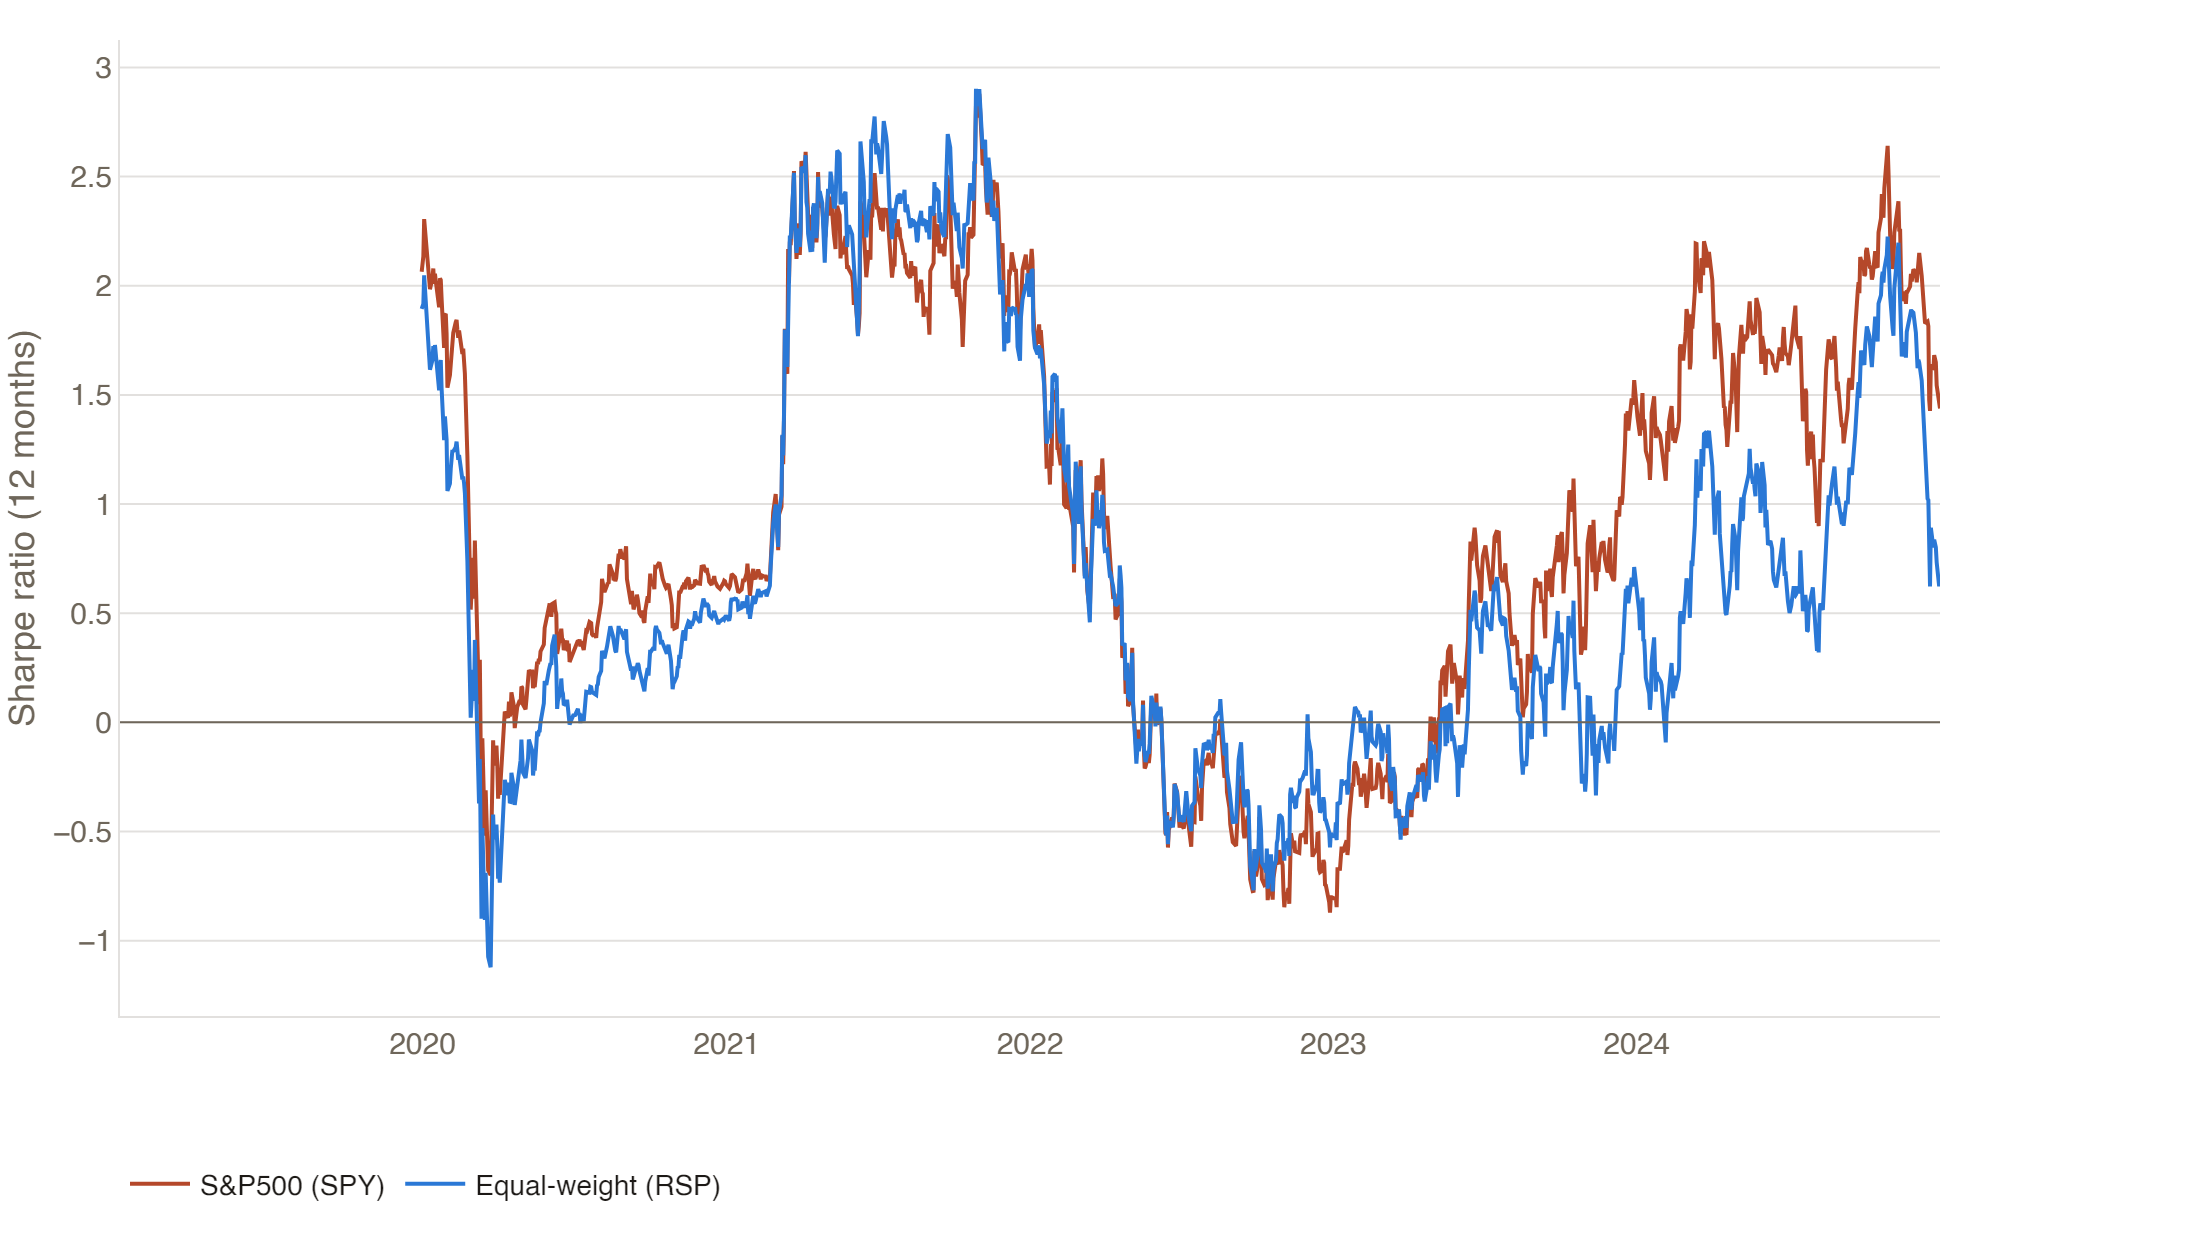
\includegraphics[width=\linewidth]{sharpe_chart.png}
  \caption{Twelve-month rolling Sharpe ratio of SPY and RSP, using the realized risk-free rate.}
  \label{fig:sharpe}
\end{figure}

The rolling Sharpe ratio (Figure~\ref{fig:sharpe}) is higher for SPY on $68\%$ of days, but not always: in 2021 and 2022 RSP had a slightly higher Sharpe ratio on average. SPY's lead is largest in 2024, with an average difference of $0.74$.

\subsection{Statistical significance}

We test the hypothesis that the mean daily return difference $d_t = r_t^{\text{SPY}} - r_t^{\text{RSP}}$ is zero, over the $1{,}509$ observations. The mean difference corresponds to $+2.95$ percentage points per year in favour of SPY, but the $t$-test does not reject the null hypothesis ($t = 1.05$, $p = 0.29$). The result does not change with Newey-West standard errors with 7 lags, which account for the autocorrelation of returns ($t = 1.06$, $p = 0.29$).

A daily advantage that is small relative to daily volatility cannot be told apart from noise, yet compounded over six years it produces a cumulative gap of $44.6$ points. SPY's outperformance is therefore economically relevant, but it is not evidence of a persistent return premium.

\section{Discussion}

\subsection{Implications for the Efficient Market Hypothesis}

The results allow two readings. Under the efficiency hypothesis, the weight reached by the Magnificent Seven reflects exceptional and correctly priced fundamentals (cloud computing, digital advertising, investment in artificial intelligence). The fact that a few well-known stocks produced most of the return is not in itself evidence of inefficiency: the semi-strong form only rules out abnormal returns obtainable from public information, and the concentration was known to everyone throughout the period. The behavioural reading, following \citet{shiller1981} and \citet{debondt1985}, would instead see signs of overreaction in the speed and size of the 2023--2024 rerating. Our data do not allow us to choose between the two: because of the joint-hypothesis problem \citep{fama1991}, the answer depends on the assumed pricing model.

\subsection{Concentration risk for passive investors}

A capitalization-weighted fund automatically buys a larger share of the stocks that rise. When large firms grow, index funds invest more in them, and the additional demand further supports their weight. Diversification, the main argument for index investing \citep{markowitz1952}, shrinks without the investor changing anything. The $44.6$-point gap between SPY and RSP measures the gain from concentration over the period; the maximum drawdown of the Magnificent Seven ($-44.0\%$) shows its risk.

\subsection{Caveats}

Three caveats limit the conclusions. First, the Magnificent Seven group is defined ex post: excluding the firms that won lowers the counterfactual index return by construction. For this reason the main comparison remains the one between SPY and RSP, which does not depend on this choice. Second, the 2019--2024 period was particularly favourable to these firms; over a different period the effect would differ. Third, if valuations are justified by fundamentals, there is no inefficiency to exploit.

\section{Conclusion}

With market capitalizations rebuilt from SEC data, a universe rebuilt every year and a real equal-weight benchmark, the S\&P500's 2019--2024 performance turns out to be largely tied to the Magnificent Seven. Within the universe of the 50 largest stocks their share rises from $29.5\%$ to $55.0\%$ and their contribution accounts for $66\%$ of the cumulative return; the capitalization-weighted index beats its equal-weight version by $44.6$ points. Concentration appears to be a structural feature of capitalization-weighted indexing, amplifying both returns and risks. Whether it reflects efficient pricing of exceptional fundamentals or excess enthusiasm cannot be decided from returns alone.

Compared with version 1 the qualitative conclusion is unchanged, but the numbers differ: concentration almost doubled rather than tripled, and the contribution of the Magnificent Seven is measured exactly.

\bibliographystyle{plainnat}
\bibliography{references}

\end{document}
